\chapter{The ATLAS Detector}

The \ac{ATLAS} detector is a cylindrical general purpose particle detector designed to measure the products of $\sqrt{s} = 14 \TeV$ proton-proton collisions at the \ac{LHC}. It consists of three major sub-detectors: closest to the beamline is the the \ac{ID}, which measures the trajectories of charge particles, followed by the Calorimeters, which measure the energies of electromagnetic and hadronically interacting particles, and finally the \ac{MS} which measures the trajectories of muons. The \ac{ID} is surrounded by a super conducting solenoidal magnet that provides a uniform $2$T magnetic field, enabling measurement of particles' charge and momentum, and a toroidal magnet surrounds \ac{MS}, allowing for charge and momentum measurements of muons. In general, each subdetector consists of a barrel detector parallel to the beampipe and end-cap detectors perpendicular to the beampipe. \cite{atlas-overview}

A schematic of the \ac{ATLAS} detector is shown in \autoref{fig:atlas-schematic}.


%https://atlas.cern/discover/detector
\begin{figure}[htbp]
\centering
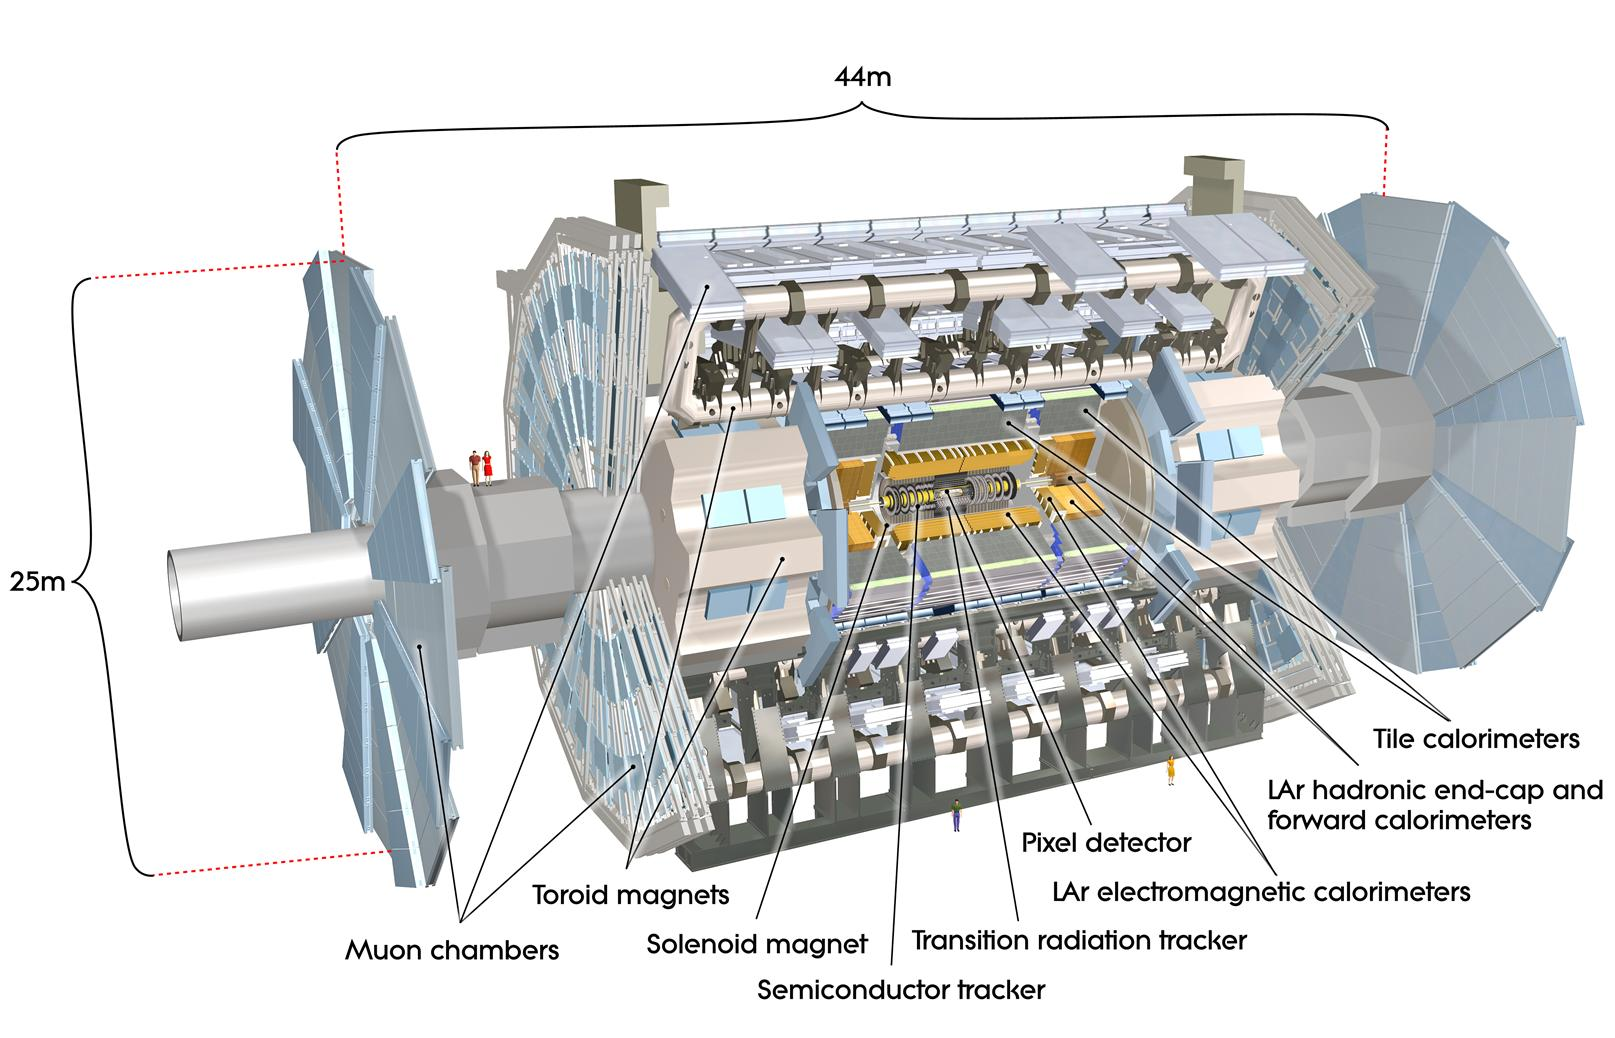
\includegraphics[width=.8\textwidth]{figures/Detector/atlas-schematic.jpg}
\caption{A diagram of the \ac{ATLAS} detector. The dimensions, subdetectors, and magnet systems are labeled. }
\label{fig:atlas-schematic}
\end{figure}

\section{Coordinate System}
\ac{ATLAS} uses a Cartesian right-handed coordinate system, with the origin defined as the $pp$ collision point. The $z$-axis points along the beampipe, where $+z$ points counter-clockwise. The transverse plane, the $y$-axis and $x$-axis, points upward and toward the center of the \ac{LHC} ring, respectively. The detector is built with with symmetry across the origin in in $z$, as well as with rotational symmetry in the transverse plane. The $+z$ side of the detector is referred to as the A-side, and $-z$ as the C-side.

Cylindrical coordinates provide a comfortable description of the \ac{ATLAS} detector, where $\phi$ measures the angle in the $x-y$ plane around the beampipe, and $\theta$ the angle from the $z$ axis. $\phi$ is positive for positive $y$. 

A given particle's momentum in $z$ is not known, but its transverse momentum is known to be $0$, so it is advantageous to define spatial variables independent of $z$ momentum. Thus, instead of $\theta$, $\eta = - \textrm{ln}(\textrm{tan}\frac{\theta}{2})$ is used to describe angle from the $z$ axis. Particles perpendicular to the $z$ axis have $\eta = 0$, while those parallel to the beamline have $\eta \rightarrow \infty$. 

Angular distances between objects is described using $\Delta R = \sqrt{\Delta \eta ^2 + \Delta \phi ^2}$ and the radial distance from the origin in the $x-y$ plane is denoted $R$. 

A particle's momentum will generally be described in terms of its \pT, its momentum in the transverse direction. A particle's $3$-vector is described by $(\pt, \eta, \phi)$, which are all invariant under boosts in $z$ assuming the particle can be considered massless (which is true in the case of particles in \ac{ATLAS}).





%USED ATLAS-overview.pdf
\section{Inner Detector}
The Inner Detector measures the trajectories of charged particles resulting from \ac{LHC} collisions. The \ac{ID} covers the region with $|\eta| < 2.5$, measuring approximately $1000$ particles per bunch crossing. In order to achieve the momentum and vertex resolution required to achieve \ac{ATLAS}'s physics goals three subdetectors are used: the Pixel detector, the \ac{SCT}, and the \ac{TRT}. The Pixel and \ac{SCT} detectors are used for high granularity precision tracking and the \ac{TRT} is used to distinguish electrons from converted photons. All of this is immersed in a $2$T magnetic field, curving charged particles in proportion to its momentum in the $\phi$ direction.

\todo{describe conversions somewhere... Maybe in particle descriptions in theory?}


The \pt resolution of the \ac{ID} scales with track \pt. Higher \pt tracks are less curved, so the measurement resolution is worse. In the \ac{ATLAS} \ac{ID}, the \pt resolution  $0.05\% \times \pt$ with a $1\%$ constant term. The constant term describes measurement uncertainties that do not scale with momentum or energy, such as material imperfections, non-uniform detector response, or other constant measurement issues and is added in quadrature ($\oplus$) with the stochastic term.

The combination of thre three trackers with radii ranging from 32.33 mm to 1082mm enable robust and precise pattern recognition. The Pixel detector enables secondary vertex measurements, and combined with the \ac{SCT} enables impact parameter measurement and vertexing for heavy-flavor jet and $\tau$-lepton tagging. the The \ac{TRT} has lower precision per point, but measures a longer track and contributes signficantly to the momentum measurement.


A schematic of the \ac{ID} can be seen in \autoref{fig:atlas-id} and a detailed distribution of the various subdetectors is shown in \autoref{fig:atlas-id-layers}. 


%https://cds.cern.ch/images/CERN-GE-0803014-01/file?size=medium
\begin{figure}[htbp]
\centering
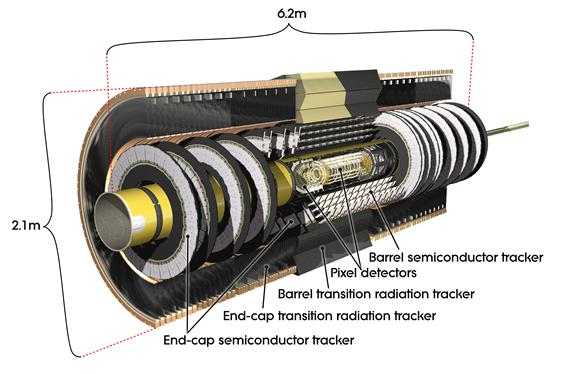
\includegraphics[width=.8\textwidth]{figures/Detector/atlas-ID.jpg}
\caption{A diagram of the \ac{ATLAS} \ac{ID} with the major subsystems labeled. The Pixel and \ac{SCT} are of particular importance for this analysis.}
\label{fig:atlas-id}
\end{figure}

%https://www.researchgate.net/publication/325643426/figure/fig8/AS:669532737769482@1536640452588/Segment-of-the-ATLAS-inner-detector-showing-the-tracker-layers-The-silicon-strip.ppm
\begin{figure}[htbp]
\centering
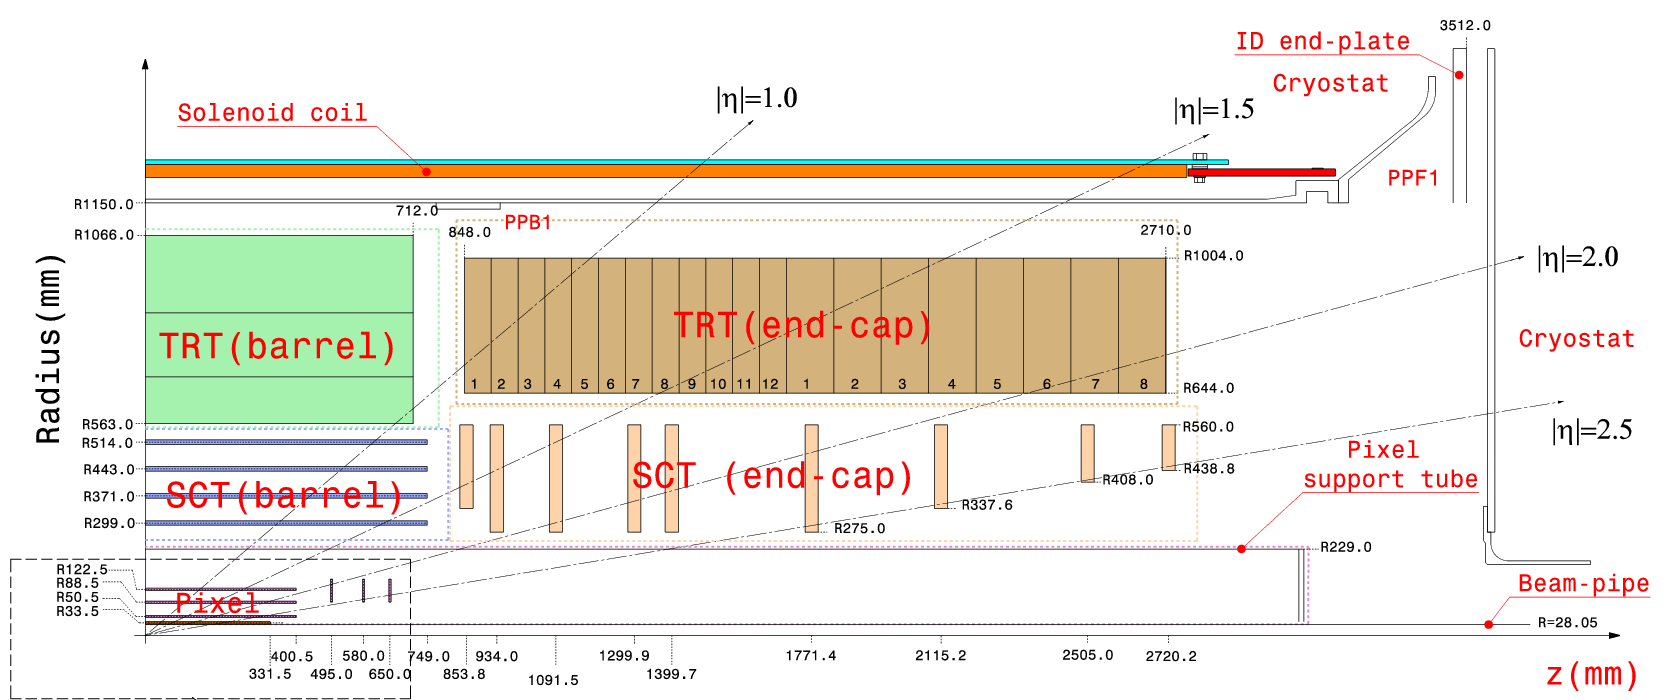
\includegraphics[width=.8\textwidth]{figures/Detector/atlas-id-layers.png}
\caption{A schematic of the \ac{ATLAS} \ac{ID} shown in the $R-z$ plane. \cite{id-cutaway}}
\label{fig:atlas-id-layers}
\end{figure}

\subsection{Silicon Detectors}



\subsection{The Pixel Detector}

The Pixel detector is the closest one to the beam and have the highest granularity. The pixels are arranged parallel to the beam axis in concentric cylindrical layers in the barrel and perpendicular to the beam axis on disks in the endcap regions. The current Pixel detector consists of the Run 1 detector with the \ac{IBL} installed closed to the beam pipe. 

The Run 1 Pixel detector has 3 concentric cylindrical layers in the barrel and 3 disks in the endcap. It is composed of 1744 pixel sensors, each with 47232 pixels. Each pixel is identical has minimum size of $R-\phi \times z = 50 \times 400 \mu \textrm{m}^{2}$ (increasing to $R-\phi \times z = 50 \times 600 \mu \textrm{m}^{2}$ near a front-end chip). In the barrel, they have accuracy of $10 \mu \textrm{m}$ in $R-\phi$ and $115 \mu \textrm{m}$ in $z$, and in the endcaps they have accuracy of $10 \mu \textrm{m}$ in $R-\phi$ and $115 \mu \textrm{m}$ in $R$ and the detector has 80.4 million pixels and readout channels. 

The \ac{IBL} is the inner most Pixel layer installed for Run 2 33.2 mm away from a new, narrower beampipe. A closer detector layer enables better impact parameter resolution as well as providing extra radiation shielding for the former closest Pixel layer (called the B-layer). The \ac{IBL} is composed of 12 million smaller pixels, $R-\phi \times z = 50 \times 250 \mu \textrm{m}^{2}$, assembled on 14 staves, with a resolution of $8 \mu\textrm{m}$ in $R-\phi$ and $40 \mu\textrm{m}$.

The two innermost detectors, the Pixel and \ac{SCT} detectors, are made of silicon, the preferred tracking medium of particle physics detectors. The \ac{ATLAS} pixels are n-type semiconductors (impurities have been added to increase the number of potential electron charge carriers) with a voltage applied (150-600V in the Pixel detector).  When a charged particle interacts with a silicon detector layer, electron-hole pairs are created and these pairs drift toward the readout chips in the magnetic field. If enough of these pairs are created such that the signal becomes greater than a pre-specified noise threshold, the signal is readout as a \emph{hit}. A particle must have 3.6 eV to induce about 80 electron-hole pairs per $\mu$m. Pixels provide a high signal-to-noise ratio, and so are preferred in regions where high occupancy is possible (such as close to the beamline). \cite{silicon} 

\subsection{The Silicon Microstrip Tracker}
A particle moving through the \ac{SCT} crosses 4 bilayers of the detector creating 4 hit measurements as it interacts with 8 layers of material. In the barrel, each bilayer is composed of 2 stereostrips, one parallel to the beam axis (measuring $R-\phi$) and the other rotated by 40 mrad. The combination of the stereostrips in the bilayer gives a 3-dimensional measurement. In the end caps, the bilayers are arranged on 9  disks per side such that the second layer is offset 40mrad from a radial strip. The strips are 12cm long and $80 \mu\textrm{m}$ thick.

Less precise than the Pixels, in the barrel region, they have accuracy of $17 \mu \textrm{m}$ in $R-\phi$ and $580 \mu \textrm{m}$ in $z$, and in the endcaps they have resolution of $17 \mu \textrm{m}$ in $R-\phi$ and $580 \mu \textrm{m}$ in $R$. The use of strips instead of pixels reduces the number of readout channels as well as the cost: there are 15192 sensors each with 768 strips with an applied voltage of 150-300V and 6.3 million readout channels 
 

\subsection{The Transition Radiation Tracker}
The \ac{TRT} is straw-tube tracker that extends the tracking volume by almost 500 mm without the cost of that much additional silicon. The tubes have a diameter of 4mm and made of Kapton and carbon fibers. They are filled with a gas mixture (70\% Xe, 27\% CO$_{2}$, and 3\% O$_{2}$) and a 31 $\mu$m diameter gold-plated tungsten wire. The wires are divided into two halves about $\eta = 0$. In the barrel, 52 544 straws are parallel to the beam axis and 144 cm long. In the endcaps, 122 880 37 cm long straws are arranged radially in wheels. The \ac{TRT} has 351,000 readout channels.

When a charged particle passes through the tube, the gas is ionized and the resulting free electrons drift toward the wire where they are amplified then readout. A particle passing through the \ac{TRT} typically leaves 36 hits. The \ac{TRT} only provides $R-\phi$ measurements with an accuracy of $130 \mu\textrm{m}$ per straw. However, its length improves measured momentum resolution and it also can provide ns-level timing information.


\subsection{Solenoid Magnet}

The central solenoid surrounds the \ac{ID} and provides a uniform $2\textrm{T}$ field that bends the trajectories of charged particles. The transverse momentum of the particle can be inferred from its radius of curvature, $R$, in the $x-y$ plane using the equation $p_{T} = qBR$, where $q$ is the charge of the particle and $B$ the magnetic field in the $z$ direction.

However, the placement of the solenoid between the \ac{ID} and calorimeters necessitates careful design choices so that all of a given particle's energy is still measured by the calorimeters. The solenoid only contributes about $0.66$ radiation lengths \footnote{Radiation lengths measure the mean distance in which an electron loses all but $\frac{1}{e}$ of its energy.}. In order to achieve this, the solenoid and \ac{EM} calorimeter share a vacuum vessel, eliminating the need for two vacuum walls. It is made of Al-stabilised NbTi superconductor which allows a high electric field to be achieved ($7.730 \textrm{kA}$) while optimizing the thickness of the coil. The solenoid has an axial length of $5.8 \textrm{m}$ and radial thickness of $100 \textrm{cm}$ and it operates at a temperature of $4.5 \textrm{K}$. 


\section{Calorimeters}

The \ac{ATLAS} calorimeters measure the energy of electromagnetic and hadronic particles. The calorimeter system is composed of \ac{EM}, hadronic, and forward calorimeters. While they use a variety of different technologies to measure energies, they are both sampling calorimeters composed of alternating active and absorbing layers. Particles shower in absorbing layers and the showers are measured in the active layers, but the actual energy of each particle is not measured because some is lost to the absorbing layers. Unlike the tracker, the energy resolution of a calorimeter increases with increasing energy due to the increased signal generated. The size of each calorimeter is set by its radiation length or nuclear interaction length such that the calorimeter absorbs all of given particle's energy by the far end of the calorimeter and only muons and neutrinos should escape the calorimeters layers. A schematic of the \ac{ATLAS} calorimeters can be seen in \autoref{fig:atlas-calos}


%https://arxiv.org/pdf/1603.02934.pdf
\begin{figure}[htbp]
\centering
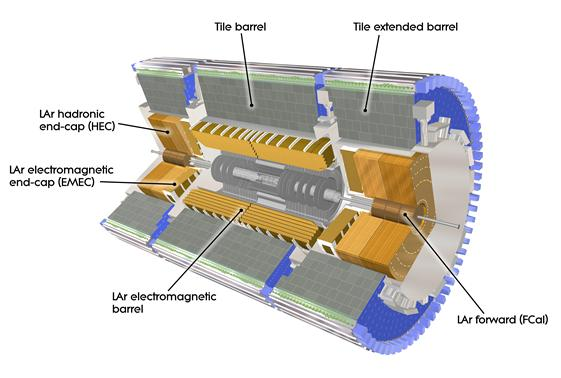
\includegraphics[width=.8\textwidth]{figures/Detector/atlas-calorimeters.jpg}
\caption{A diagram of the \ac{ATLAS} calorimeters with the major subsystems labeled. The \ac{EM} calorimeter is of particular importance for this analysis. \cite{calorimeters}}
\label{fig:atlas-calos}
\end{figure}


\subsection{Electromagnetic Calorimeter}

The \ac{LAr} \ac{EM} calorimeter is the innermost calorimeter and gives excellent energy and position resolution. \cite{calorimeters} It is composed of barrel ($|\eta| < 1.5$) and end-cap ($1.4 < |\eta| < 3.2$) components. Both components use a lead absorber with liquid argon active material. The layers of the calorimeter have an accordion shape (shown in \autoref{fig:atlas-lar}), which allows for the multiple absorbing layers without any gaps between them, as well as complete $\phi$ symmetry. The first layer has finer segmentation in $\eta$ to allow for more precise angular measurements of photons (which do not produce an \ac{ID} track). The thickness of the absorbing plates varies as a function of $\eta$ to optimize energy resolution. An active liquid argon presampler is placed before the accordion layers in the region with $|\eta| < 1.8$ to correct for energy loss upstream of the calorimeter. It is about 22 radiation lengths wide and gives energy resolution of $10\%/\sqrt{E} \oplus 0.7\%$

%https://www.researchgate.net/profile/Denis_Oliveira_Damazio/publication/229849719/figure/fig2/AS:667635272413188@1536188061121/Calorimeter-cells-for-different-layers-left-Note-the-very-fine-segmentation-in-the_Q320.jpg
\begin{figure}[htbp]
\centering
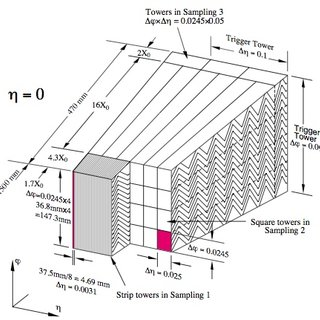
\includegraphics[width=.6\textwidth]{figures/Detector/lar.jpg}
\caption{A diagram of the \ac{ATLAS} \ac{EM} \ac{LAr} calorimeter. It has a unique shape in order to provide precision position and energy resolution.}
\label{fig:atlas-lar}
\end{figure}


\subsection{Hadronic Calorimeter}

The hadronic calorimeter surrounds the \ac{EM} calorimeter also within $|\eta| < 3.2$. The barrel region ($|\eta| < 1.7$) is made of steel absorbers with active material of scintillating tiles. Here, the calorimeter is about $2$m long in the radial direction and covers about $8$ interaction lengths. The Hadronic End-cap Calorimeters cover the region $1.5 < |\eta| < 3.2$ with a copper absorber and liquid argon active material.


The hadronic calorimeter has an energy resolution of  $50\%/\sqrt{E} \oplus 3\%$. 

\subsection{Forward Calorimeter}
The \ac{FCAL} is measures  both \ac{EM} and hadronic energy and extends coverage to $3.1 < |\eta| < 4.9$. The detector uses liquid argon as its active material with copper (for \ac{EM} activity) and tungsten (for hadronic activity) absorbers. It is about $10$ interaction lengths deep and also serves to add some shielding to the \ac{MS}. The energy resolution of the \ac{FCAL} is $100\%/\sqrt{E} \oplus 10\%$.




\section{Muon Spectrometer}
The Muon Spectrometer is the outermost subdetector designed to detect muons, which are too massive to be stopped by the calorimeters, and measure their momentum. This is achieved using a toroidal magnet system that deflects muons as they pass through through  high-precision tracking chambers and separate chambers used for triggering. The magnetic field points in the $\eta$ direction, orthogonal to the muon's direction of motion, and the detector as well as the toroid system is symmetric in $\phi$.

The \ac{MS} can measure muons with $|\eta| < 2.4$ and $3 \GeV < {\pt}_{\mu} < 10 \TeV$. The main performance goal is to provide a stand-alone (independent of the \ac{ID}) momentum resolution of $10\%$ at $\pT > 1 \TeV$; a particle moving with $\pt = 1 \TeV$ has a \emph{sagitta} (see \autoref{fig:ms-sagitta}) of $500\mu\textrm{m}$ that needs to be measured with a resolution of $<50\mu\textrm{m}$. Even at 3 \TeV, the \ac{MS} has good momentum resolution and is still able identify the charge of the particle based on its bending direction. Furthermore, the triggering chambers have timing resolution of $1.5-4 \textrm{ns}$.  

\begin{figure}[htbp]
\centering
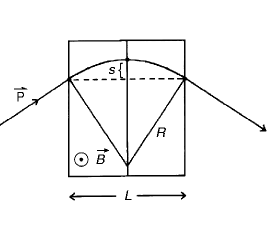
\includegraphics[width=.6\textwidth]{figures/Detector/ms-sagitta.png}
\caption{The trajectory of a particle in a magnetic field (``B''). The particle's sagitta, labeled ``s'' is the bending distance in the direction perpendicular to the magnetic field. The direction of the bending is dictated by the charge of the particle. The higher the momentum of a particle, the smaller the sagitta. \cite{particledetectors-springer}}
\label{fig:ms-sagitta}
\end{figure}


\ac{MDT}s are used for precision tracking in the $\eta$ coordinate in the range $|\eta| < 2.7$, except in the inner most layer where the \ac{MDT}s extend only to $|\eta| < 2.0$ and \ac{CSC}s cover the region $2.0|\eta| < 2.7$. Triggering and $\phi$ measurements are provided by \ac{RPC}s in the range $|\eta| < 1.05$ and \ac{TGC}s in $1.05 |\eta| < 2.7$. The detector chambers are arranged in concentric cylindrical shells around the beam axis at radii of about 5m, 7.5m and 10m in the barrel, and on wheels perpendicular to the beam axis at distances of about 7.4m, 10.8m, 14m, and 21.5m from the interaction point. There is a gap in detector coverage around $|\eta| = 0$ for detector access for service work. A schematic of the \ac{MS} can be seen in \autoref{fig:atlas-ms}.  

\begin{figure}[htbp]
\centering
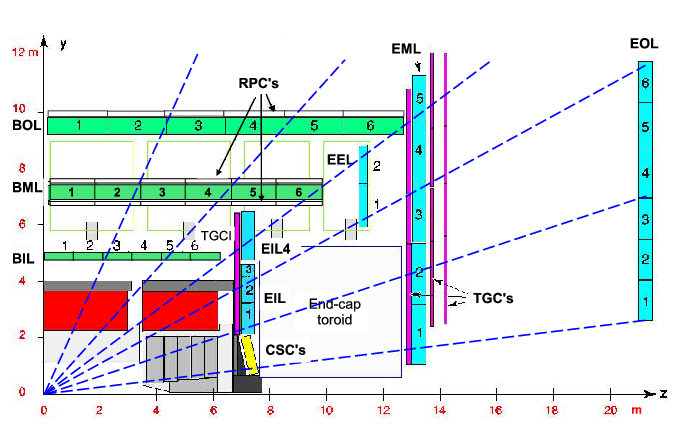
\includegraphics[width=.6\textwidth]{figures/Detector/atlas-ms.png}
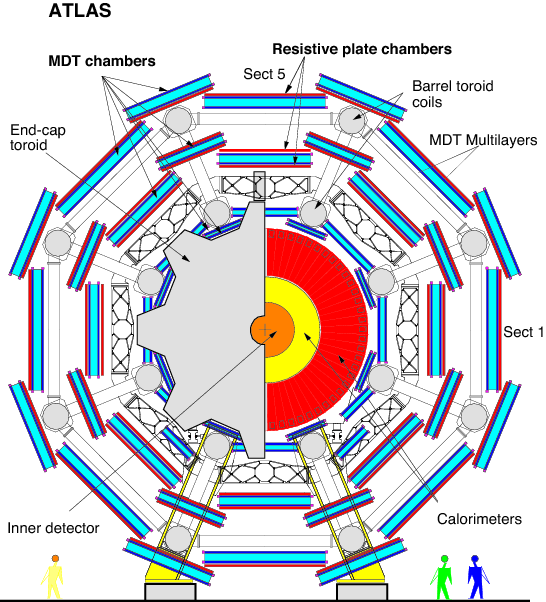
\includegraphics[width=.3\textwidth]{figures/Detector/mdt-phi.png}
\caption{A diagram of the \ac{ATLAS} \ac{MS} in the $r-z$ (left) plane and a $\phi$ cross section of the barrel region. On the left, the barrel \ac{MDT} are shown in green and the \ac{RPC} shown in black. In the end-caps, the \ac{MDT} are shown in blue and the \ac{TGC} shown in purple. On the right, the concentric cyclindrical layers of \ac{MDT}s are shown: 8 small chambers and 8 large chambers. The diameter is 20m at its widest. \cite{ms-vertices}}
\label{fig:atlas-ms}
\end{figure}


While the \ac{MDT}s give extremely precise measurements of muon directions, they cannot be used in isolation for the physics goals of \ac{ATLAS}. First, they are finely segmented in $\eta$, the bending direction of the muons, enabling the high momentum resolution. However, in $\phi$, their resolution is as good as the length of the tube, several meters long. Additionally, being drift tubes, their readout is very slow and cannot be used in the quick response time required for triggering. Thus, \ac{RPC}s (in the barrel) and \ac{TGC}s (in the endcaps) complement the \ac{MDT}s for triggering and \ac{CSC}s complement the \ac{MDT}s in the forward region (where the particle flux is the highest) to provide better 2-dimensional position measurements. A comparison of the resolution of the different detectors of the \ac{MS} can be seen in \autoref{tab:ms-parts}. 

\begin{table}[htb]
\begin{center}
\begin{tabular}{ccccc}
Detector    & function & z/R resolution & $\phi$ resolution & time resolution \\
 \hline
  \ac{MDT}  &  tracking   &  35 \um (z)  & 2.5-5 m  & $<$ 700 ns \\
  \ac{CSC}  &  tracking   &  30 \um (R)  & 5 mm     & 7 ns   \\
  \ac{RPC}  &  triggering &  10 mm  (z)  & 10 mm    & 1.5 ns  \\
  \ac{TGC}  &  triggering &  2-6 mm (R) & 3-7 mm   & 4 ns  \\
\hline
\end{tabular}
\caption{Resolutions of the various parts of the \ac{MS}. The endcap detectors (\ac{CSC}s and \ac{TGC}s) give resolution in R while the barrel detectors (\ac{MDT}s and \ac{RPC}s) give resolution in z. The various pieces of the \ac{MS} enable 2 dimensional precision measurement as well as measurements to be used in the trigger.}
\label{tab:ms-parts}
\end{center}
\end{table}

\subsection{Monitored Drift Tubes and Cathode-Strip Chambers}

The fundamental unit of the \ac{MDT} chambers are 30mm diameter pressurized drift tubes. Each drift tube is filled with Ar/CO$_{2}$ gas and a 50 \um diameter tungsten-rhenium wire. When a muon passes through the tube, it ionizes electrons from the atoms in the gas. These electrons travel along the electric field in the tube until they reach the positively charged wire. The location of the electrons along the wire give a position measurement. The time of arrival of the first charges at the wire determine the radius of the drift-circle, seen in \autoref{fig:ms-drift} If the muon itself passes close to the wire during its trajectory it can induce a signal in the wire, so a dead time is specified before the detector readout. The spatial resolution of a single drift tube is 80 \um. 

Each \ac{MDT} chamber consists of two multilayers of drift tubes separated by a mechanical spacer. The inner chambers, where the highest performance is required, a multilayer is composed of four layers of drift tubes (increasing the resolution to 35 \um), while the middle and outer chambers multilayers are composed of three layers (increasing the resolution to 30 \um). The combination of the three chambers gives the required sagitta resolution with about 15 measurements per muon. There are 1150 \ac{MDT} chambers with 354,000 drift tubes. The tubes cannot bend more than 100\um, a significant challenge against gravity. The tubes are held in tension and carefully calibrated and monitored to achieve a maximum bending of 20 \um. 

The \ac{CSC}s are multiwire proportional chambers with anode wires oriented radially. The wires are held between two cathodes: one segmented with strips perpendicular to the wires giving a precision measurement in the bending plane ($\eta$) of with resolution of 40\um and the other segmented parallel to the wire, giving a transverse ($\phi$) measurement with 5mm resolution. The signals from the wires are not readout, rather a position is obtained by measuring the relative charge deposited on neighboring strips. The \ac{CSC}s are segmented into chambers in $\phi$, each consisting of four layers, resulting in four measurements per muon.


\subsubsection{MDT Timing}
\label{sec:mdt-timing}
The readout of the \ac{MDT}s also gives a profile of the hits that compose the signal in time, seen in \autoref{fig:ms-t0fit}. The peak of the distribution, $t_{0}$, measures the time the signal began with respect to $t=0$, the time of the $pp$ interaction measured by the \ac{ATLAS} clock. The end of the signal, $t_{\text{max}}$, is the maximum drift time. In a perfectly calibrated detector, the $t_{0}$ measurement is Gaussian about $t_{0} = 0$ with a width of about 3ns. 



\begin{figure}[htbp]
\centering
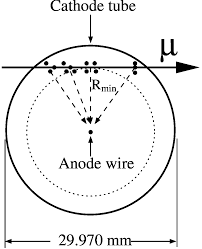
\includegraphics[width=.6\textwidth]{figures/Detector/ms-drift.png}
\caption{A sketch of a muon passing through a cross section of an \ac{MDT}. \cite{atlas-overview}}
\label{fig:ms-drift}
\end{figure}

\begin{figure}[htbp]
\centering
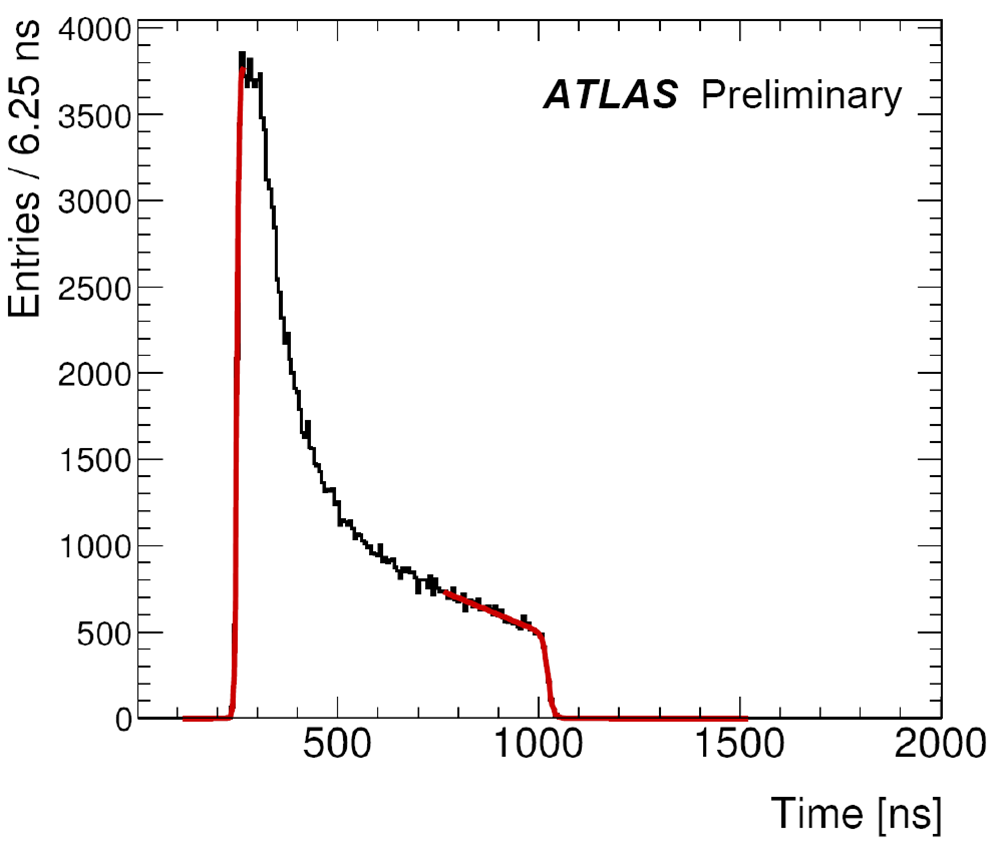
\includegraphics[width=.6\textwidth]{figures/Detector/mdt-t0.png}
\caption{A distribution of \ac{MDT} time measurements. The $t_{0}$ is the time between 0 and the peak of the distribution, shown by the leftmost red line. The rightmost red line indicates $t_{\textrm{max}}$, the end of the \ac{MDT} signal. \cite{muon-public}}
\label{fig:ms-t0fit}
\end{figure}




\subsection{Resistive Plate Chambers and Thin Gap Chambers}

The trigger chambers must provide transverse momentum resolution in the barrel and endcaps over the full $\phi$ range, have time resolution such that detector information can be matched to the correct bunch crossing, be robust against photon and neutron backgrounds in the experimental cavern, and provide a $\phi$ measurement to complement the \ac{MDT} $\eta$ measurement.


In the barrel, \ac{RPC}s are used to achieve these goals. An \ac{RPC} is a parallel plate detector composed of two phenolic-melaminic plastic laminate plates 2mm apart filled with C$_{2}$H$_{2}$F$_{4}$ gas and with a 4.9 kV/mm field between them. When a muon passes through the detector, it ionizes the atoms in the gas, the ionized electrons further ionize other atoms, creating an avalanche. Both sides of the chamber are readout; they have perpendicular readout strips, giving both $z$ and $\phi$ measurements. The \ac{RPC}s are arranged into chambers of two detector layers each (giving two measurements per chamber) and positioned above or below each \ac{MDT} chamber.

In the endcaps, multiwire proportional chamber \ac{TGC}s are used. They work very similarly to the \ac{CSC}s, with perpendicular anode wires and cathode strips, but the unit is more compact, giving the requisite increase in speed. Multiwire proportional chambers are ideal for the endcaps of the \ac{MS} because have an extremely granular readout, which allows them to deal well with the inhomogeneity of the magnetic field in the transition region.


\subsection{Toroid Magnets}

The toroid magnet system, composed of a barrel and two end-caps, provides a toroidal magnetic field of $0.5 \textrm{T}$ and $1 \textrm{T}$ for the barrel ($|\eta| < 1.4$) and end-cap ($1.6 <|\eta| < 2.7$) regions of the \ac{MS}. In the transition region ($1.5 < |\eta| < 1.6$) muons are bent by a combination of the two fields resulting in an extremely heterogeneous field making accurate measurement challenging. This inhomogeneity results in geometric regions where the muon trajectories are not bent at all, mimicking a high \pt muon, adding challenges for triggering on high \pt muons in this region. The toroid is much larger than the solenoid, $25.3 \textrm{m}$ long and $10 \textrm{m}$ in radial width, but also operates at a temperature of $4.5 \textrm{K}$. All three toroid magnets are made of Al-stabilized Nb/Ti/Cu conductor. They have an air-core structure, which gives them a strong bending power over a large volume while minimizing material that could induce any additional scattering. 




\section{Particles in ATLAS}
The previously described subdetectors are used in combination to identify particles in \ac{ATLAS}. Charged particles interact with the \ac{ID} resulting in hits to be reconstructed into tracks. A track that points to a calorimeter cluster indicates the kind of charged particle that made the track and a cluster without an associated track indicates a neutral particle. The calorimeters are designed such that they absorb all of the energy of a particle and \ac{EM} particles do not enter the hadronic calorimeter, and hadronic particles do not enter the \ac{MS}. Muons do not interact with the calorimeters, but do leave a track in both the \ac{ID} and \ac{MS}. The only \ac{SM} particle that escapes the detector entirely is a neutrino. An undetected particle, like an \ac{SM} $\nu$ or some \ac{BSM} particle, could be seen as an imbalance in transverse momentum. The transverse momenta of all particles should sum to zero in order to conserve momentum, so any non-zero sum indicates an undetected particle.


\begin{figure}[htbp]
\centering
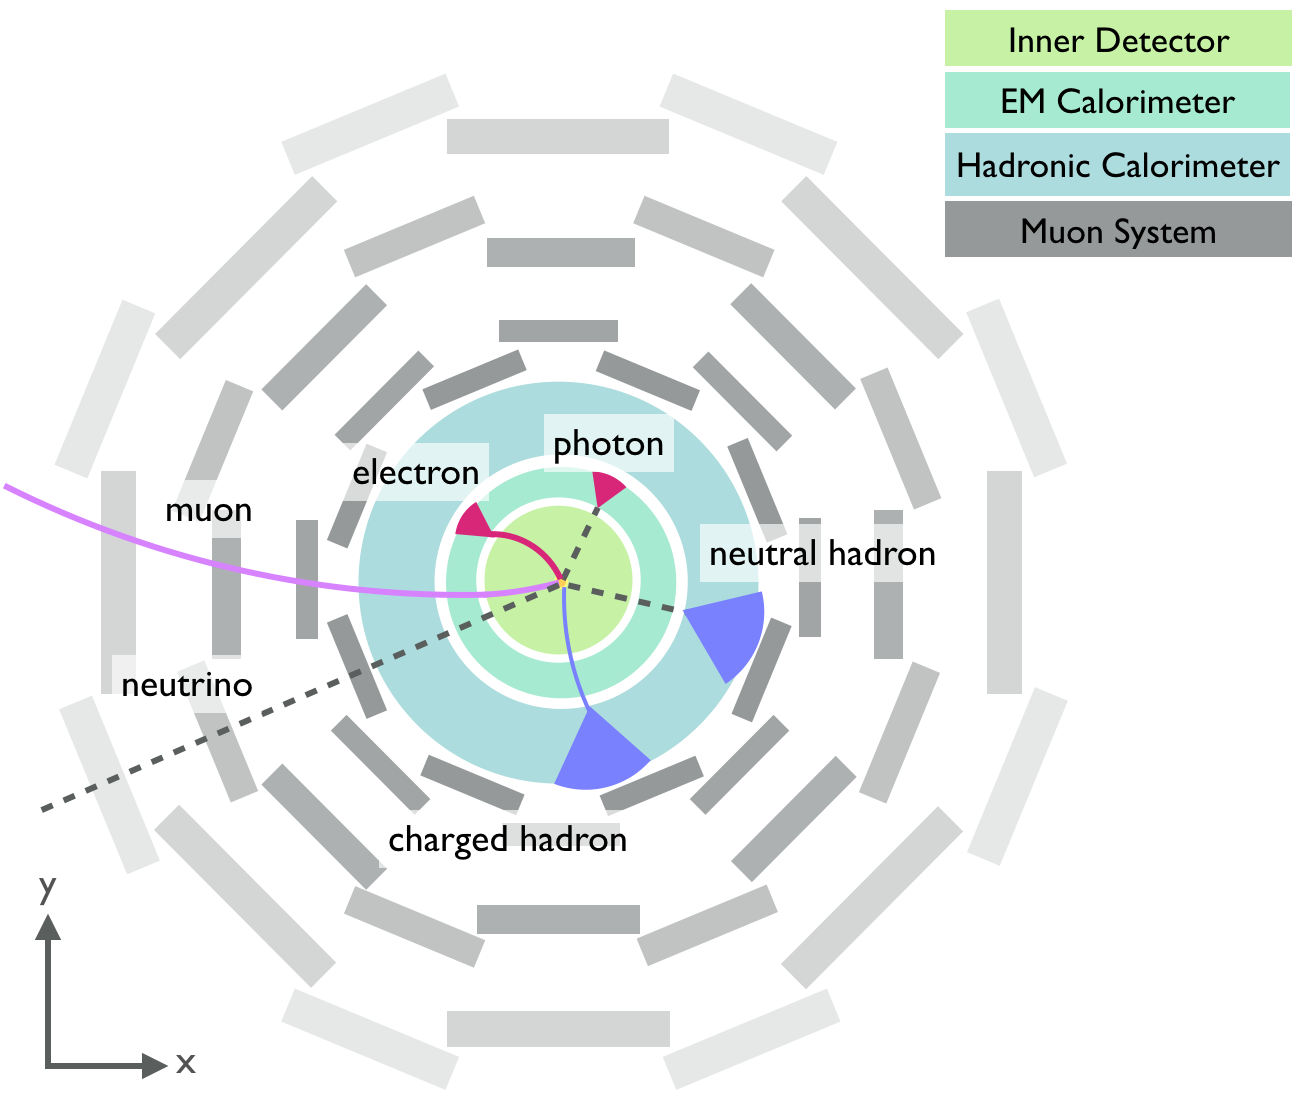
\includegraphics[width=.8\textwidth]{figures/Detector/particle-doodle.png}
\caption{A schematic of the signatures of Standard Model particles in the \ac{ATLAS} detector that illustrates how the subdetectors are used together to identify particles. Dashed lines indicate a particle trajectory that leaves no detector signature. Figure not drawn to scale nor does it represent a real physical process.}
\label{fig:particle-doodles}
\end{figure}




